\noindent\textbf{Dificultad:} Media

\subsection{Descripción del nivel}
El binario solicita un nombre de usuario y un serial de 8 dígitos hexadecimales. El serial se calcula a partir del usuario, por lo que el objetivo es reconstruir esa función y escribir un \emph{keygen}.

\begin{figure}[H]
\centering
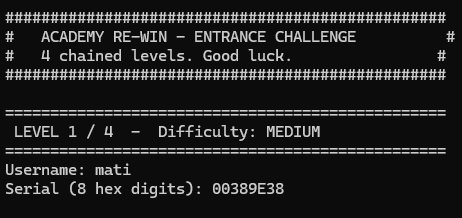
\includegraphics[width=0.7\linewidth]{initial/img/level1.png}
\caption{Pantalla del nivel 1: usuario y serial ingresados}
\label{fig:level1}
\end{figure}

\subsection{Análisis estático}
% Cómo se ubicó la rutina de validación: cadenas, referencias cruzadas, funciones relevantes.
\textit{[A completar.]}

\subsection{Análisis dinámico}
% Breakpoints usados, registros/memoria observados en la comparación.
\textit{[A completar.]}

\subsection{Algoritmo de validación}
% Pseudocódigo del algoritmo reconstruido.
\textit{[A completar.]}

\subsection{Solución (keygen)}
\textit{[A completar.]}

\begin{lstlisting}[language=Python]
# Keygen - Nivel 1
# TODO: pegar el código del keygen
\end{lstlisting}

\subsection{Resultado}
El binario acepta la credencial: la entrada se ve en la Figura~\ref{fig:level1} y el mensaje \texttt{Level 1 PASSED} al comienzo de la Figura~\ref{fig:level2}.

\begin{lstlisting}[language={}]
Username: mati
Serial: 00389E38
[+] Level 1 PASSED
\end{lstlisting}
